
\documentclass[a4paper,12pt]{article}

% Packages
\usepackage{graphicx}
\usepackage{float}
\usepackage[margin=1in]{geometry}
\usepackage{caption}

\begin{document}

\title{GitHub Repository Insights Analysis}
\author{}
\date{\today}

\maketitle

\section{GitHub Repository Insights}

This section presents the visual analysis of the repository's
contribution activity, commit history, code frequency, and
contributor statistics using the GitHub Insights data.

% Figure 1: Contributors
\begin{figure}[H]
    \centering
    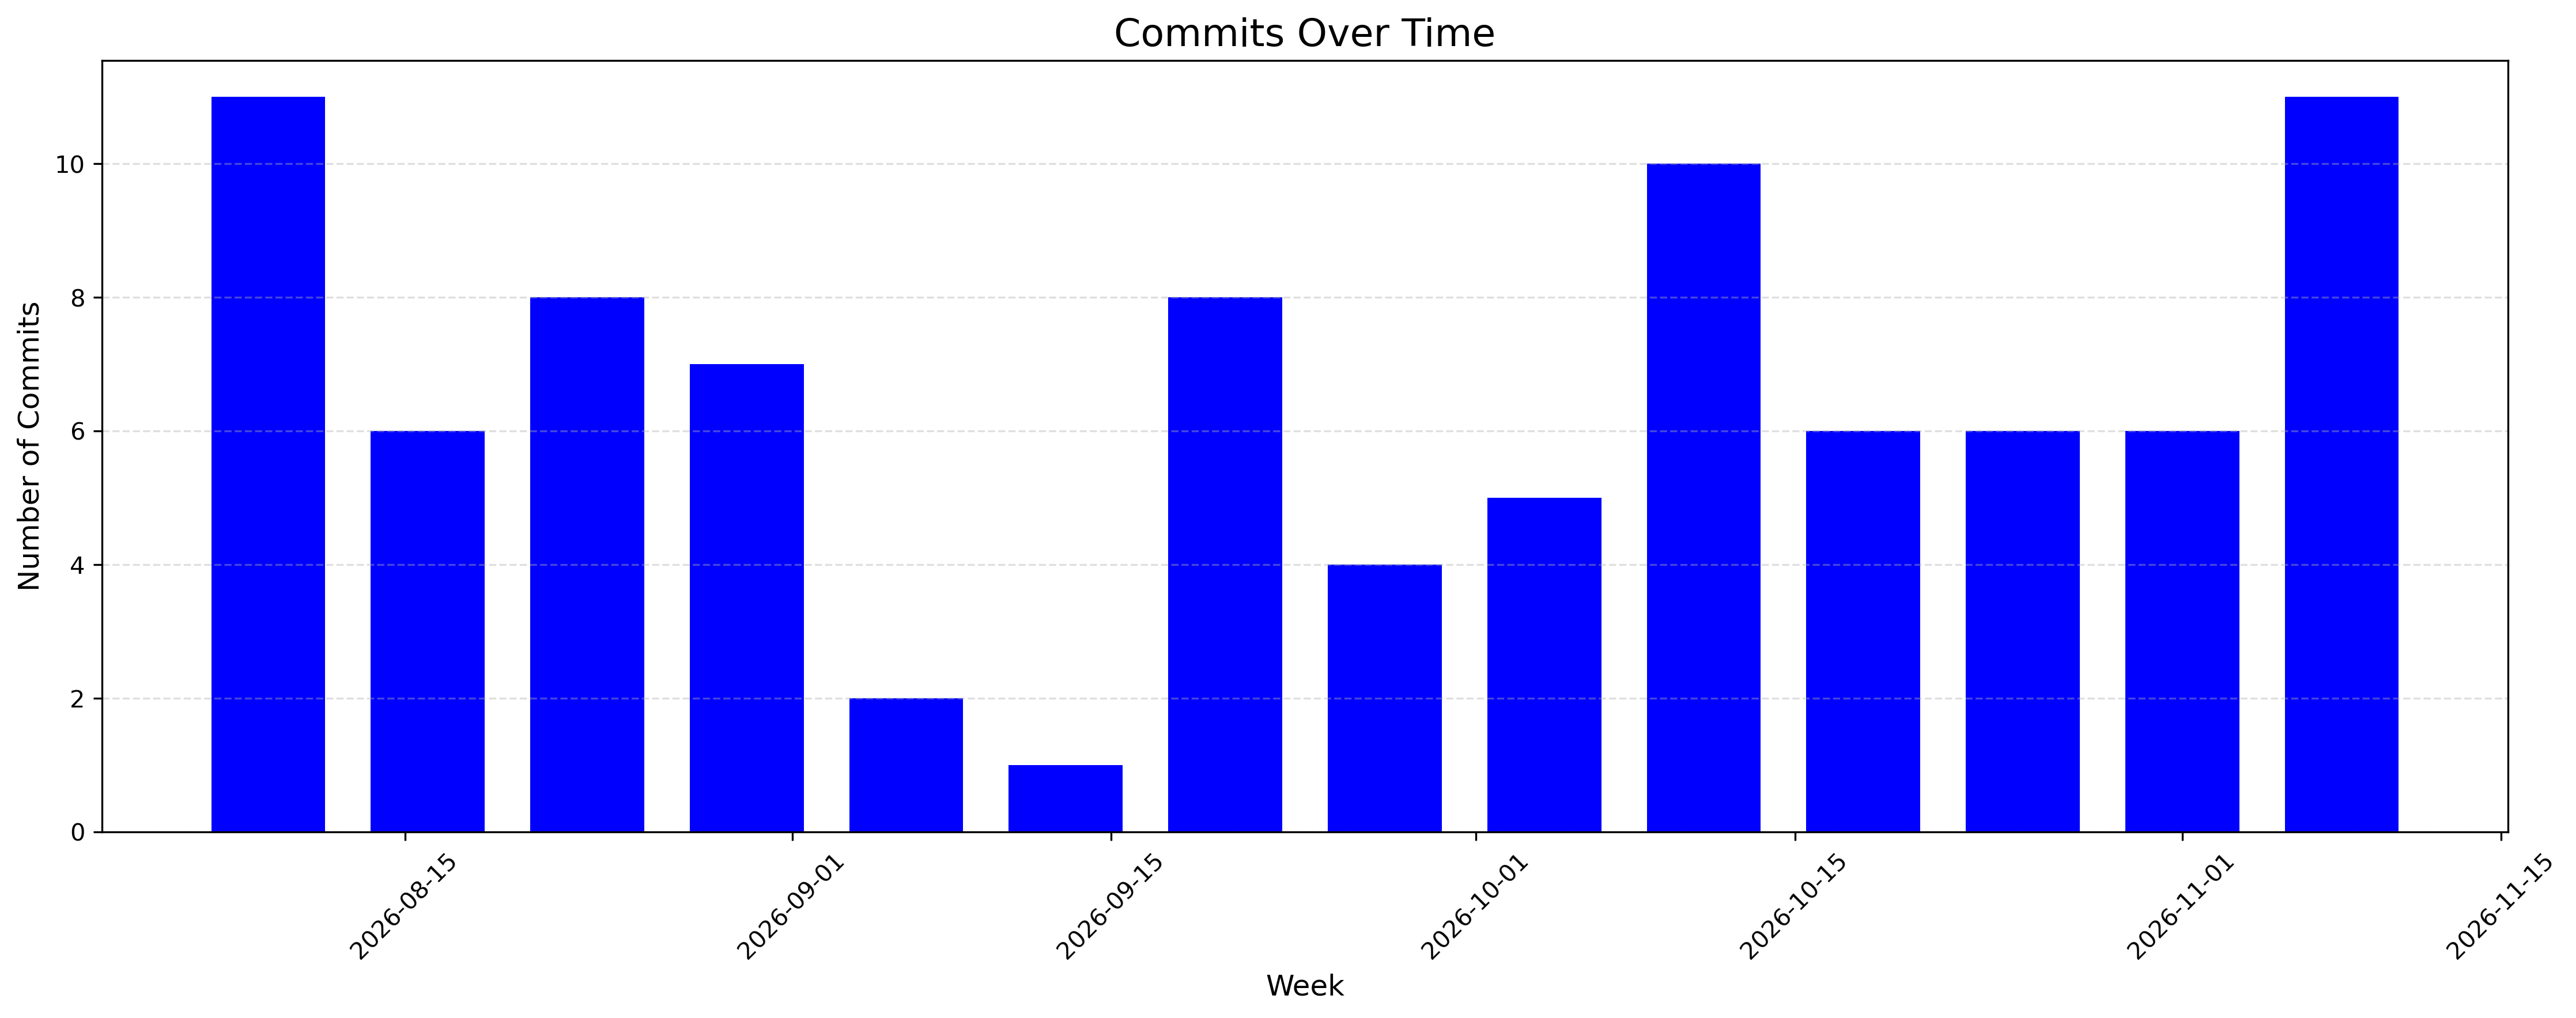
\includegraphics[width=0.95\textwidth]{fig-1/fig1.png}
    \caption{Commits over time per contributor, showing the
    weekly contribution activity of individual contributors.}
    \label{fig:contributors}
\end{figure}

% Figure 2: Commits
\begin{figure}[H]
    \centering
    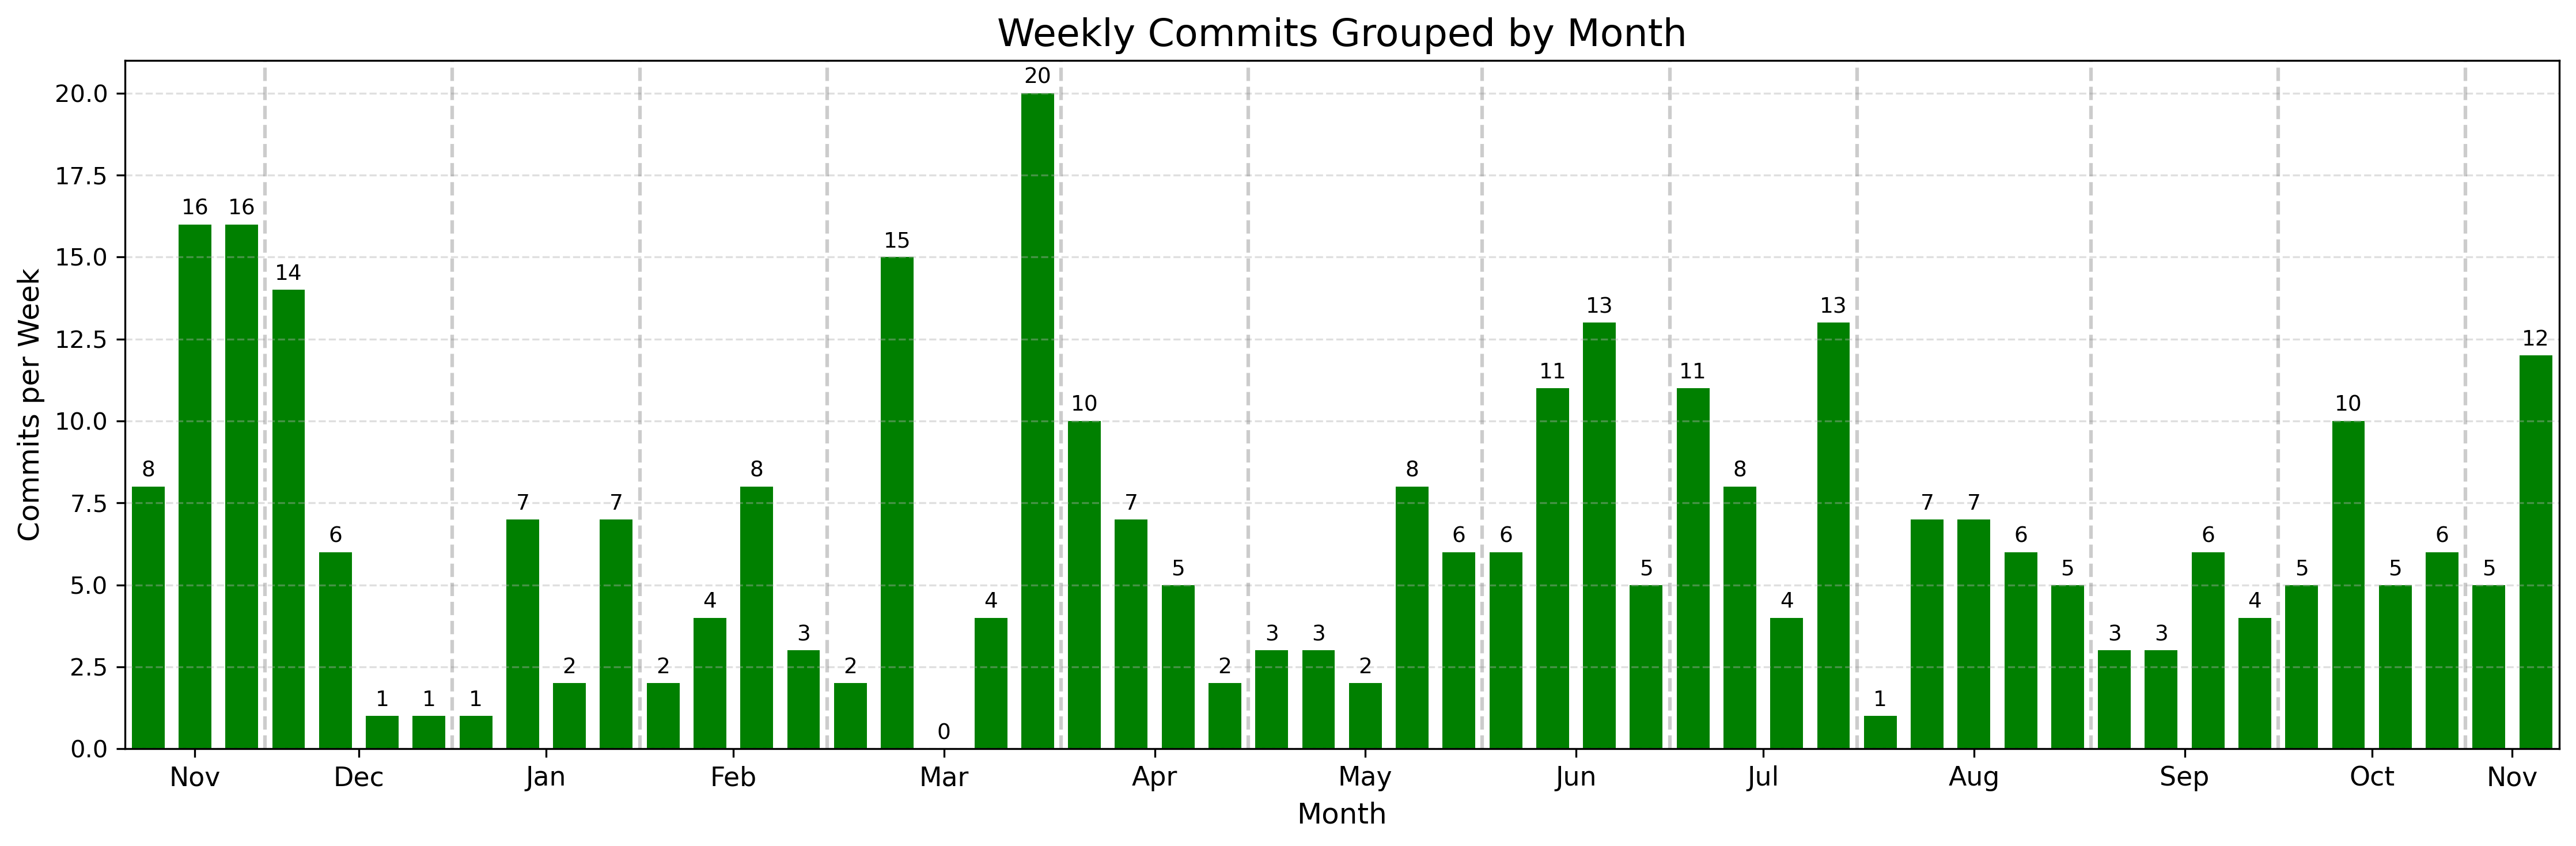
\includegraphics[width=0.95\textwidth]{fig-2/fig2.png}
    \caption{Commits per week, illustrating the repository's
    weekly commit activity over time.}
    \label{fig:commits}
\end{figure}

% Figure 3: Code Frequency
\begin{figure}[H]
    \centering
    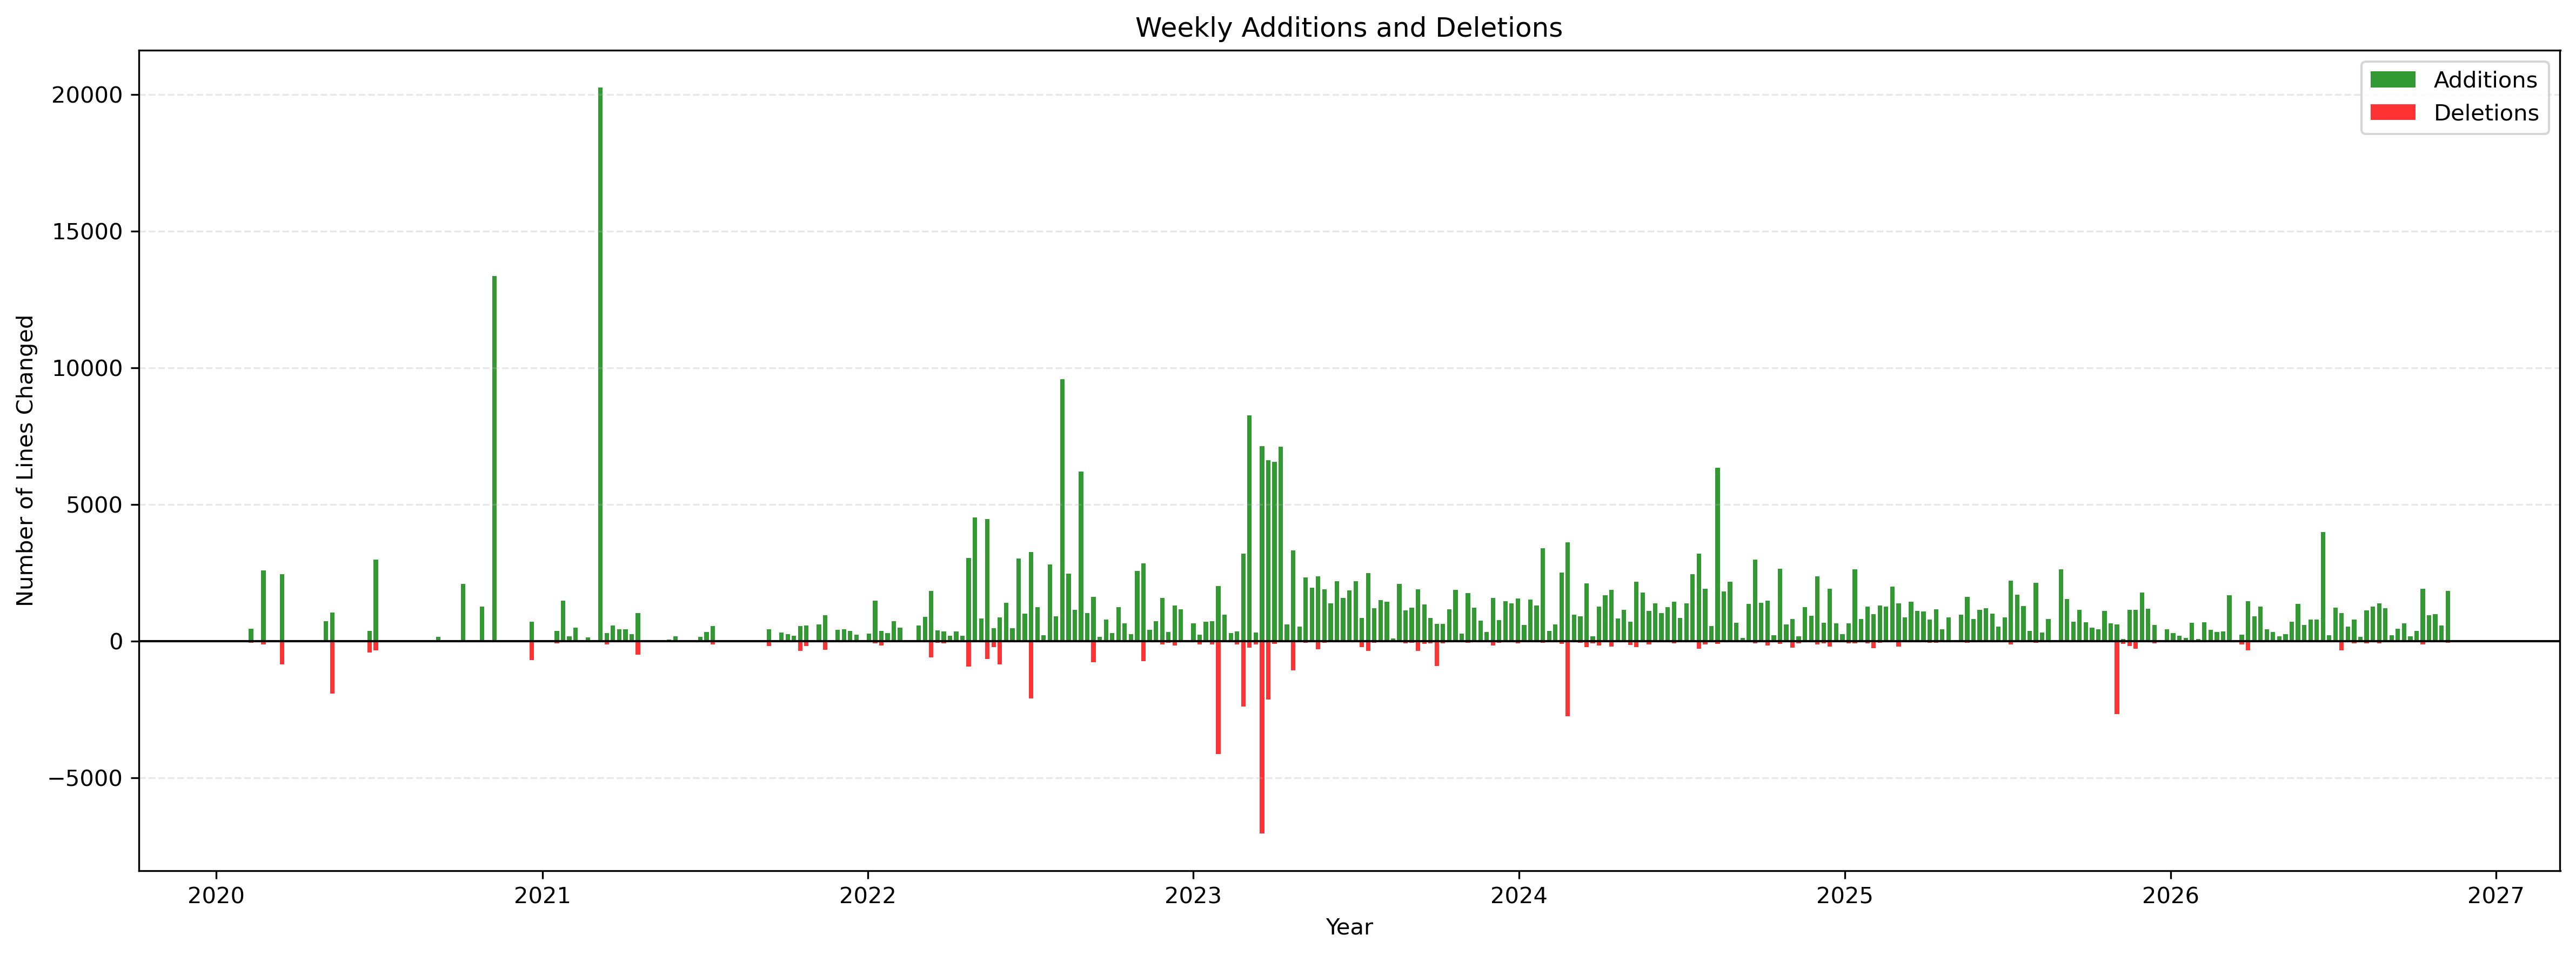
\includegraphics[width=0.95\textwidth]{fig-3/fig3.png}
    \caption{Weekly code frequency, representing the number
    of lines of code added and deleted over time.}
    \label{fig:code-frequency}
\end{figure}

% Figure 4: Top Committers
\begin{figure}[H]
    \centering
    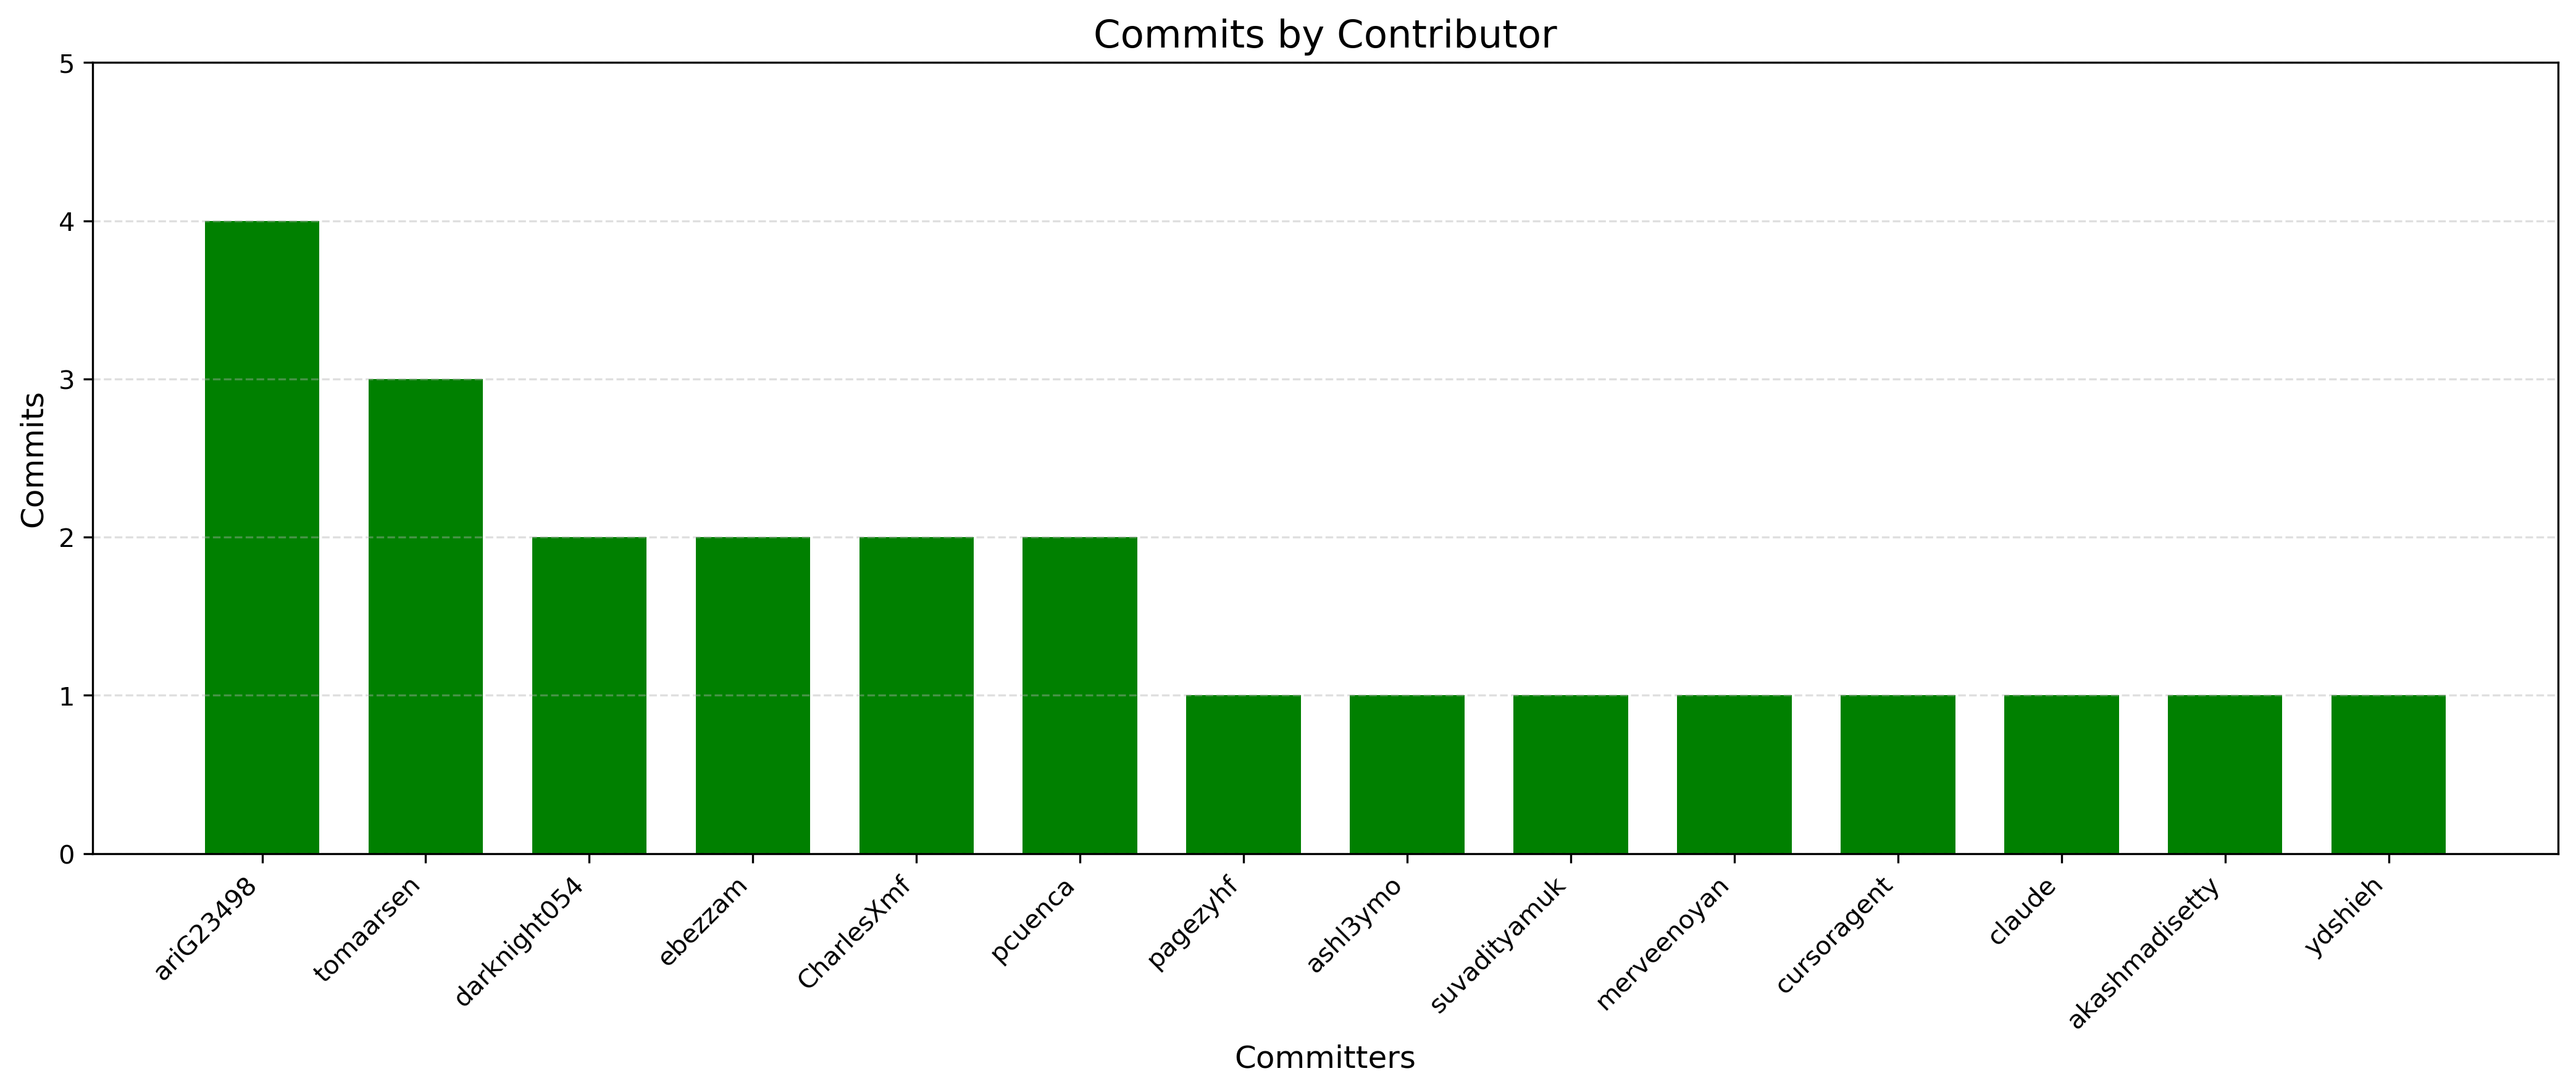
\includegraphics[width=0.95\textwidth]{fig-4/fig4.png}
    \caption{Top committers in the repository, ranked by the
    total number of commits contributed by each author.}
    \label{fig:top-committers}
\end{figure}

\section{Conclusion}

The four figures provide an overview of repository development
activity, highlighting individual contributions, weekly commit
trends, code additions and deletions, and the most active
contributors.

\end{document}
